
\section{维数、超越次数与\trNoetherNormalization}

现在，我们将为\trIrreducible\trVariety{}的\trDimension{}给出另一种强有力的解读，即用\trTrDeg{}来表述。其证明将涉及一个经典的构造——\trNoetherNormalization（Noether normalization），它在别的方面也大有用处。倘若你还没见识过超越理论（transcendence theory），这里有一份闪电式的介绍。

\textbf{12.2.A.（练习／定义）}\quad 回想：\trFieldExtension{} $E/F$ 的一个元素称为在 $F$ 上\trAlgebraic{}的，如果它在 $F$ 上\trIntegral。还要回想：\trFieldExtension{} $E/F$ 称为一个\trAlgebraic\trFieldExtension，如果它是一个\trIntegralExtension{}（即 $E$ 的全部元素都在 $F$ 上\trAlgebraic{}的；参看 \S8.2）。由\cref{ex:integrality-composition}，两个\trAlgebraic\trFieldExtension{}的\trComposition{}仍是\trAlgebraic{}的。设 $E/F$ 是一个\trFieldExtension，而 $F'$ 与 $F''$ 是两个中间\trFieldExtension，则只要 $F'F''$ 在 $F'$ 与 $F''$ 之上都是\trAlgebraic{}的，我们就写 $F'\sim F''$。这里的 $F'F''$ 是 $F'$ 与 $F''$ 的\textbf{\trCompositum}（compositum），即 $E$ 中同时含有 $F'$ 与 $F''$ 的最小\trFieldExtension。
\begin{enumerate}[label=(\alph*)]
  \item 证明：$\sim$ 是 $E/F$ 的诸子扩张上的一个\trEquivalenceRelation。$E/F$ 的一个\textbf{\trTranscendenceBase}（transcendence basis）是一组元素 $\{x_i\}$：它们在 $F$ 上\textbf{\trAlgebraicallyIndependent}（algebraically independent）（即诸 $x_i$ 之间不存在系数取自 $F$ 的非平凡多项式关系），并且满足 $F(\{x_i\})\sim E$。
  \item 证明：若 $E/F$ 有两个\trTranscendenceBase，而其中之一的基数为 $n$，则两者的基数都是 $n$。（提示：证明你可以把其中一个基里的元素逐个换入另一个基。）任何\trTranscendenceBase{}的大小都称为\textbf{\trTrDeg}（transcendence degree，可以是 $\infty$），记作 $\operatorname{trdeg}$。任何\trFinitelyGenerated{}的\trFieldExtension{}必有有限的\trTrDeg。（注记：有关的结果见定理~10.5.17。）
\end{enumerate}

\textbf{12.2.1.\ \trhTheorem{}（\trDimension{}＝\trTrDeg）。}\ ——\ \emph{设 $A$ 是域 $k$ 上\trFinitelyGenerated{}的\trIntegralDomain{}（即一个\trFinitelyGenerated{}的 $k$-\trAlgebra，而且是\trIntegralDomain）。那么 $\dim\Spec A=\operatorname{trdeg}K(A)/k$。从而若 $X$ 是\trIrreducible{} $k$-\trVariety，则 $\dim X=\operatorname{trdeg}K(X)/k$。}

我们很快就会证明定理~12.2.1（\S12.2.7）。在此之前，先给出几个直接的推论，以展示它的用处。看起来我们立刻就有 $\dim\mathbb{A}^n_k=n$。然而，我们对定理~12.2.1 的证明恰好要\emph{经过}这一事实，所以它其实算不上推论。

一个更有分量的推论如下。若 $X$ 是\trIrreducible{} $k$-\trVariety，则 $\dim X$ 就是\trFunctionField{}（即\trGenericPoint{}处的\trStalk）$\OO_{X,\eta}$ 在 $k$ 上的\trTrDeg。于是（由于\trGenericPoint{}落在一切非空\trOpenSet{}之中）\trDimension{}可以在 $X$ 的任何\trOpenSet{}中计算。（\trhWarning{}：去掉\trFiniteType{}假设后这就不真了，哪怕在相当合理的情境中也是如此——取 $X$ 为两点空间 $\Spec k[x]_{(x)}$，并让 $\mathsf{U}$ 仅由\trGenericPoint{}组成；见\cref{ex:topological-space-kx-p}。）

另一个推论，是\trNullstellensatz{}（\cref{thm:hilbert-nullstellensatz}）的第二个证明。

\textbf{12.2.B.（练习：由维数论到\trNullstellensatz）}\quad 设 $A=k[x_1,\dots,x_n]/I$。证明：$A$ 的任何\trMaximalIdeal{}的\trResidueField{}都是 $k$ 的一个\trFiniteFieldExtension。（提示：诸\trMaximalIdeal{}对应于\trDimension{}为 $0$ 的点，而这些点又对应于 $k$ 的\trTrDeg{}为 $0$ 的\trFinitelyGenerated\trExtension，也就是 $k$ 的\trFiniteFieldExtension。）

还有一个推论则颇合几何直觉。

\textbf{12.2.C.（练习）}\quad 若 $\pi\colon X\to Y$ 是\trIrreducible{} $k$-\trVariety{}之间的一个\trDominant{}\trMorphism，则 $\dim X\ge\dim Y$。（更一般的情形下这不真：考虑把\trGenericPoint{}含入一条\trIrreducible\trCurve{}的\trInclusionMap。）

\textbf{12.2.D.（练习）}\quad 设 $f_1(x_1,\dots,x_n),\dots,f_m(x_1,\dots,x_n)\in k[x_1,\dots,x_n]$ 是某个域上 $n$ 个变量的 $m$ 个多项式，其中 $m>n$。证明：多项式 $f_1,\dots,f_m$ 是\trAlgebraicallyDependent{}的（algebraically dependent）。（注记：若 $m=n$，你怎样才能判断诸 $f_i$ 是否\trAlgebraicallyIndependent？在\trCharacteristic{} $0$ 时有一个异乎寻常地简单的答案：诸 $f_i$ \trAlgebraicallyDependent，当且仅当\textbf{\trJacobianMatrix}（Jacobian matrix）的\trDeterminant{}是零多项式；见\mbox{练习~21.6.C}！这在\trCharacteristic{} $p$ 时不真：若 $f_i(x_1,\dots,x_n)=x_i^p$，则诸 $f_i$ \trAlgebraicallyIndependent，然而\trJacobianMatrix{}是零矩阵。）

\textbf{12.2.E.（练习：为操练概念而设）}\quad 证明：下面三个方程
\[
wz-xy=0,\qquad wy-x^2=0,\qquad xz-y^2=0
\]
在 $\mathbb{A}^4_k$ 中切出一个\trIntegral{}的\trSurface{} $S$。（这几个方程你或许认得，出自\cref{ex:twisted-cubic-cone}与\mbox{练习~9.3.A}。）你也许会以为 $S$ 是一条\trCurve，因为它是在四维空间中由三个方程切出的。可行的方法之一（办法多得很）：把 $S$ 切成小块。例如，证明 $D(w)\cong\Spec k[x,w]_w$。（你或许认得 $S$：它是\trTwistedCubic{}上的\trAffine\trCone。那个\trTwistedCubic{}定义于\mbox{练习~9.3.A}。）结果你需要三个方程才能切出这张\trSurface。第一个方程在 $\mathbb{A}^4_k$ 中切出一个三维\trVariety（依据\trKrull{}主理想定理~12.3.3，我们很快就会与它见面）。第二个方程切出一张\trSurface：我们的\trSurface，连同另一张\trSurface。第三个方程切出我们的\trSurface，并把「多余的分量」除掉。最后顺带一提：请再次注意，\trQuadricSurface{} $k[w,x,y,z]/(wz-xy)$ 上的\trCone{}又露面了。

\textbf{12.2.2.\ \trhDefinition{}：\trIrreducible\trVariety{}的\trRationalMap{}之\trDegree。}\quad 若 $\pi\colon X\dashrightarrow Y$ 是同\trDimension{}的\trIrreducible（从而\trIntegral）$k$-\trVariety{}之间的一个\trDominant{}\trRationalMap，则该\trFieldExtension{}的\trDegree{}称为这个\trRationalMap{}的\textbf{\trDegree}（degree）。若 $X$ 可约，这也容易推广：把 $X$ 的每个\trIrreducibleComponent{}上的\trDegree{}加起来即可。若 $\pi$ 是同\trDimension{}的\trIntegral{}仿射 $k$-\trVariety{}之间的\trRationalMap{}而不\trDominant，我们就说\trDegree{}为 $0$。在 \S24.5.14 中，我们将借「数一数 $Y$ 的\trGeneralPoint{}的原像个数」来解读这个\trDegree。注意：\trDegree{}在\trComposition{}下是乘性的：若 $\rho\colon Y\dashrightarrow Z$ 是同\trDimension{}的\trIntegral{} $k$-\trVariety{}之间的\trRationalMap，则 $\deg(\rho\circ\pi)=\deg(\rho)\deg(\pi)$，因为\trFieldExtension{}的\trDegree{}在塔中是乘性的。

\textbf{12.2.3.\ \trNoetherNormalization。}

我们对定理~12.2.1 的证明将用到另一个重要的经典观念——\trNoetherNormalization。

\textbf{12.2.4.\ \trNoetherNormalization{}引理。}\ ——\ \emph{设 $A$ 是域 $k$ 上\trFinitelyGenerated{}的\trIntegralDomain。若 $\operatorname{trdeg}K(A)/k$ 为 $n$，则存在元素 $x_1,\dots,x_n\in A$，它们在 $k$ 上\trAlgebraicallyIndependent，使得 $A$ 是 $k[x_1,\dots,x_n]$ 的\trFinite\trExtension{}（从而由推论~8.2.2，是\trIntegralExtension）。}

这个结果背后的几何内容是：给定任何\trIntegral{}的\trFiniteType{}仿射 $k$-\trScheme{} $X$，都能找到满的有限\trMorphism{} $X\to\mathbb{A}^n_k$，其中 $n$ 是 $X$ 的\trFunctionField{}（在 $k$ 上）的\trTrDeg。满性由 Lying Over 定理~8.2.5 得到；特别地，见\mbox{练习~12.1.F}。这一解读有时称为\textbf{几何\trNoetherNormalization}（geometric Noether normalization）。（\trNoetherNormalization{}的射影版本见注记~29.3.7。）

\textbf{12.2.5.\ \trNoetherNormalization{}引理~12.2.4 的\trNagata{}证明。}\quad 不妨设 $A=k[y_1,\dots,y_m]/\mathfrak{p}$，也就是说，可以选得让 $A$ 具有 $m$ 个生成元。注意 $m\ge n$。我们对 $m$ 作归纳来证明结果。基底情形 $m=n$ 是显然的。

现在设 $m>n$，并且结果对更小的 $m$ 已经证得。我们将找出 $A$ 的 $m-1$ 个元素 $z_1,\dots,z_{m-1}$，使得 $A$ 在 $k[z_1,\dots,z_{m-1}]/\mathfrak{q}$ 上有限（即：$A$ 的由 $z_1,\dots,z_{m-1}$ 生成的\trSubring，其中诸 $z_i$ 满足由\trIdeal{} $\mathfrak{q}$ 给出的那些关系）。于是由归纳假设，$k[z_1,\dots,z_{m-1}]/\mathfrak{q}$ 在某个 $k[x_1,\dots,x_n]$ 上有限，而 $A$ 在 $k[z_1,\dots,z_{m-1}]$ 上有限，故由\mbox{练习~8.3.H}，$A$ 在 $k[x_1,\dots,x_n]$ 上有限。
\[
\begin{tikzcd}[row sep=3.2em]
A=k[y_1,\dots,y_m]/\mathfrak{p} \ar[d, no head, "\text{有限}"] \\
k[z_1,\dots,z_{m-1}]/\mathfrak{q} \ar[d, no head, "\text{有限}"] \\
k[x_1,\dots,x_n]
\end{tikzcd}
\]
由于 $y_1,\dots,y_m$ 在 $A$ 中\trAlgebraicallyDependent，它们之间有一条非零的代数关系 $f(y_1,\dots,y_m)=0$（其中 $f$ 是 $k$ 上 $m$ 个变量的一个多项式）。

令 $z_1=y_1-y_m^{r_1}$，$z_2=y_2-y_m^{r_2}$，…，$z_{m-1}=y_{m-1}-y_m^{r_{m-1}}$，其中 $r_1,\dots,r_{m-1}$ 是马上就要选定的正整数。于是
\[
f\bigl(z_1+y_m^{r_1},\,z_2+y_m^{r_2},\,\dots,\,z_{m-1}+y_m^{r_{m-1}},\,y_m\bigr)=0.
\]
把上式展开后，$f$（视作 $m$ 个变量的多项式）的每个\trMonomial{}都将给出单独的一项：某个常数乘以 $y_m$ 的一个幂（不带 $z_i$ 因子）。只要选得诸 $r_i$ 满足 $0\ll r_1\ll r_2\ll\cdots\ll r_{m-1}$，就能保证出现的 $y_m$ 的幂两两不同，从而特别地存在一个首项 $y_m^N$，而其余各项（包括带 $z_i$ 因子的那些）在 $y_m$ 上的次数都更低。于是我们便描述了 $y_m$ 对 $z_1,\dots,z_{m-1}$ 的一条整依赖关系，正合所需。\hfill$\square$

\textbf{12.2.6.\ \trNagata{}证明背后的几何。}\quad 这里便是\trNagata{}论证背后的几何直觉。设我们在 $\mathbb{A}^m_k$ 中有一条 $n$ 维\trVariety，其中 $n<m$，例如 $\mathbb{A}^2$ 中的 $xy=1$。一个自然的指望是：到一张\trHyperplane{}的投射会是有限\trMorphism。就 $xy=1$ 而言，若投射到 $x$-轴，它就不有限，粗略地说，因为渐近线 $x=0$ 使这个\trMap{}无法保持闭性（参看\mbox{练习~8.3.K}）。如果我们转而投射到一条随机的直线，我们或许指望能摆脱这个问题，而且通常确实能：出问题的方向只有有限多个。但若域是有限的，我们可能就有麻烦了：也许可供投射的方向本就只有有限多个，偏偏个个都出了问题。（你可以证明：若 $k$ 是无限域，则上述证明中的代换 $z_i=y_i-y_m^{r_i}$ 可换成线性代换 $z_i=y_i-a_iy_m$，其中 $a_i\in k$，并且只要诸 $a_i$ 取自某个非空\trZariski\trOpenSet，我们确实就得到一个有限\trMorphism。）\trNagata{}的一般的诀窍，是把变量以非线性的方式「抖一抖」，而这一抖就杀掉了该\trMap{}的不有限性。

\textbf{12.2.F.（练习：\trFiniteType{} $k$-\trScheme{}之积的\trDimension{}可加性）}\quad 若 $X$ 与 $Y$ 都是\trIrreducible{} $k$-\trVariety，证明 $\dim X\times_k Y=\dim X+\dim Y$。提示：倘若我们有满的有限\trMorphism{} $X\to\mathbb{A}^{\dim X}_k$ 与 $Y\to\mathbb{A}^{\dim Y}_k$，我们就能构造出一个满的有限\trMorphism{} $X\times_k Y\to\mathbb{A}^{\dim X+\dim Y}_k$。（\trhWarning{}：去掉\trFiniteType{}假设后这可以不真；见注记~12.2.17。）

特别地，当 $A$ 在一个域上\trFinitelyGenerated{}时，我们有 $\dim A[x]=\dim A+1$。（当 $A$ \trNoetherian{}时，这在更一般的情形下也真，尽管我们不去证明它。）

\textbf{12.2.G.（较不重要但好玩的练习）}\quad
\begin{enumerate}[label=(\alph*)]
  \item 设 $X\subset\mathbb{P}^n$ 是一个\trIrreducible{}的射影 $k$-\trVariety。证明：$X$ 上的\trAffine\trCone{}与\trProjective\trCone{}的\trDimension{}都是 $\dim X+1$。
  \item 证明：$k[x_0,\dots,x_n]$ 中在某个\trHomogeneous{}\trIdeal{}之上极小的\trPrimeIdeal{}也是\trHomogeneous{}的。
  \item 设 $\mathfrak{p}\subset\mathfrak{q}$ 是 $k[x_0,\dots,x_n]$ 的两个\trHomogeneous{}\trPrimeIdeal，且两者之间不存在严格介于其间的\trHomogeneous{}\trPrimeIdeal。证明：两者之间也不存在严格介于其间的（不必\trHomogeneous{}的）\trPrimeIdeal。
\end{enumerate}

\textbf{12.2.7.\ 关于\trDimension{}与\trTrDeg{}的定理~12.2.1 之证明。}\quad 设 $X$ 是一个\trIntegral{}的\trFiniteType{}仿射 $k$-\trScheme。我们来证明：$\dim X$ 等于其\trFunctionField{}的\trTrDeg{} $n$，证明对 $n$ 作归纳。（想法是：我们从 $X$ 化归到 $\mathbb{A}^n$，再到 $\mathbb{A}^n$ 中的一张\trHypersurface，再到 $\mathbb{A}^{n-1}$。）设结果对所有小于 $n$ 的\trTrDeg{}已知。

由\trNoetherNormalization{}引理~12.2.4，存在满的有限\trMorphism{} $X\to\mathbb{A}^n_k$。由\mbox{练习~12.1.F}，$\dim X=\dim\mathbb{A}^n_k$。若 $n=0$，则大功告成，因为 $\dim\mathbb{A}^0_k=0$。

现在我们用归纳法证明：对 $n>0$ 有 $\dim\mathbb{A}^n_k=n$。显然 $\dim\mathbb{A}^n_k\ge n$，因为我们能描述一条长度为 $n$ 的\trIrreducible{}子集链：若 $x_1,\dots,x_n$ 是 $\mathbb{A}^n$ 上的坐标，考虑 $k[x_1,\dots,x_n]$ 中的\trIdeal{}链
\[
(0)\subset(x_1)\subset\cdots\subset(x_1,\dots,x_n).
\]
设我们有一条长度至少为 $n+1$ 的\trPrimeIdeal{}链：
\[
(0)=\mathfrak{p}_0\subset\cdots\subset\mathfrak{p}_m.
\]
取 $\mathfrak{p}_1$ 的任意一个非零元素 $g$，并令 $f$ 是 $g$ 的落在 $\mathfrak{p}_1$ 中的任意一个\trIrreducible{}因子。然后把 $\mathfrak{p}_1$ 换成 $(f)$。（当然，$\mathfrak{p}_1$ 本来也可能就是 $(f)$。）于是 $K\bigl(k[x_1,\dots,x_n]/(f(x_1,\dots,x_n))\bigr)$ 的\trTrDeg{}为 $n-1$，故由归纳法，
\[
\dim k[x_1,\dots,x_n]/(f)=n-1,
\]
从而 $\dim k[x_1,\dots,x_n]\le n$，证明完成。\hfill$\square$

\textbf{12.2.8.\ 对\trIrreducible\trVariety{}而言，\trCodimension{}是\trDimension{}之差。}\quad \trNoetherNormalization{}将帮我们证明：对\trIrreducible\trVariety{}而言，\trCodimension{}是\trDimension{}之差，也就是说，不等式~\eqref{eq:codim-dim-inequality} 总取等号。

\textbf{12.2.9.\ \trhTheorem{}。}\ ——\ \emph{设 $X$ 是\trPureDimensional{}的\trLocally\trFiniteType{} $k$-\trScheme{}（例如一个\trIrreducible{} $k$-\trVariety），$Y$ 是一个\trIrreducible\trClosedSubset，而 $\eta$ 是 $Y$ 的\trGenericPoint。那么 $\dim Y+\dim\OO_{X,\eta}=\dim X$。从而由\mbox{练习~12.1.J}，$\dim Y+\operatorname{codim}_XY=\dim X$——不等式~\eqref{eq:codim-dim-inequality} 总取等号。}

证明它正好给了我们一个机会，来介绍几个有用的观念，例如\trIntegrallyClosed{}\trIntegralDomain{}的\trFinite\trExtension{}的 Going-Down 定理（定理~12.2.12）。在开始证明之前，先给出一个代数转述。

\textbf{12.2.H.（练习）}\quad 称环 $A$ 是\textbf{\trCatenary{}的}（catenary），若对每一对嵌套的\trPrimeIdeal{} $\mathfrak{p}\subset\mathfrak{q}\subset A$，每条「从 $\mathfrak{p}$ 到 $\mathfrak{q}$」的严格递增\trPrimeIdeal{}链都含于某条极大的这种链中，并且所有极大的链都有相同的（有限）长度。（这个词我们日后不会正经用到。）证明：若 $A$ 是域 $k$ 上一个\trFinitelyGenerated{}环的\trLocalization，则 $A$ 是\trCatenary{}的。

\textbf{12.2.10.\ \trhRemark{}。}\quad 代数几何中自然冒出来的环大多是\trCatenary{}的。重要的例子包括：\trFinitelyGenerated{} $\mathbb{Z}$-代数的\trLocalization；完备\trNoetherian{}\trLocalRing；\trDedekind{}\trIntegralDomain（\S13.5.11）；以及 \trCM{}环（见 \S26.2.13）。想给出一个非\trCatenary{}环的例子却相当困难；例如可参看 [Stacks, tag 02JE] 或 [He]。

\textbf{12.2.11.\ 定理~12.2.9 之证明。}

\begin{figure}[htbp]
\centering
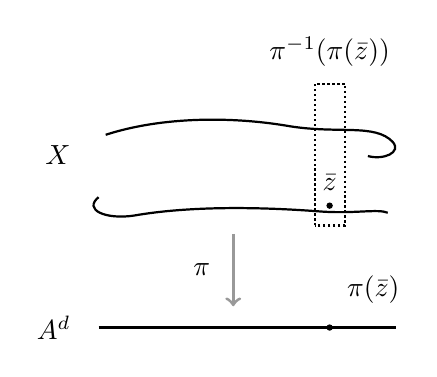
\begin{tikzpicture}[scale=0.9,line width=0.8pt]
  \draw (-1.6,1.30) .. controls (-0.8,1.56) and (0.2,1.56) .. (1.0,1.42)
        .. controls (1.7,1.31) and (2.2,1.46) .. (2.45,1.20)
        .. controls (2.58,1.05) and (2.32,0.94) .. (2.10,1.00);
  \draw (-1.70,0.42) .. controls (-1.92,0.24) and (-1.60,0.10) .. (-1.20,0.16)
        .. controls (-0.40,0.30) and (0.60,0.28) .. (1.40,0.22)
        .. controls (1.90,0.18) and (2.24,0.26) .. (2.38,0.20);
  \draw[densely dotted] (1.35,0.02) rectangle (1.78,2.02);
  \fill (1.56,0.30) circle (0.045);
  \node at (1.56,0.62) {$\bar{\boldsymbol{z}}$};
  \node[anchor=south] at (1.56,2.12) {$\pi^{-1}(\pi(\bar{\boldsymbol{z}}))$};
  \node[anchor=east] at (-1.95,1.02) {$X$};
  \draw[gray!80,line width=1.1pt,->] (0.20,-0.10) -- (0.20,-1.12);
  \node[anchor=east] at (0.02,-0.60) {$\pi$};
  \draw (-1.70,-1.42) -- (2.50,-1.42);
  \fill (1.56,-1.42) circle (0.045);
  \node[anchor=south west] at (1.66,-1.22) {$\pi(\bar{\boldsymbol{z}})$};
  \node[anchor=east] at (-1.95,-1.42) {$\mathbb{A}^d$};
\end{tikzpicture}
\caption{定理~12.2.9 之证明中的关键一步。（依原书手绘图重绘。）}\label{fig:going-down-key-step}
\end{figure}

\textbf{12.2.I.（练习）}\quad 把定理~12.2.9 的证明化归为下述问题。设 $X$ 是一个\trIrreducible{}仿射 $k$-\trVariety，而 $Z$ 是一个\trIrreducible{}的\trClosedSubset，它在所有比 $X$ 小者之中极大（唯一比 $X$ 大的\trIrreducible\trClosedSubset{}就是 $X$ 本身），那么 $\dim Z=\dim X-1$。

为方便起见令 $d=\dim X$。由\trNoetherNormalization~12.2.4，我们有对应于环的一个\trFinite\trExtension{}的有限\trMorphism{} $\pi\colon X\to\mathbb{A}^d$。于是 $\pi(Z)$ 是 $\mathbb{A}^d$ 的一个\trIrreducible\trClosedSubset（有限\trMorphism{}是闭的，\mbox{练习~8.3.L}）。

\textbf{12.2.J.（练习）}\quad 证明：只需证 $\pi(Z)$ 是一张\trHypersurface。（提示：任何\trHypersurface{}的\trDimension{}都是 $d-1$，依据的是关于\trDimension{}与\trTrDeg{}的定理~12.2.1。\mbox{练习~12.1.F}蕴涵 $\dim\pi^{-1}(\pi(Z))=\dim\pi(Z)$。但要当心：一般而言 $Z$ 并不是 $\pi^{-1}(\pi(Z))$。）

现在，若 $\pi(Z)$ 不是\trHypersurface，则它真含于一张\trIrreducible\trHypersurface{} $H$ 之中，于是由\trIntegrallyClosed{}\trIntegralDomain{}的\trFinite\trExtension{}的 Going-Down 定理~12.2.12（我们马上就来证明它），存在 $X$ 的某个真包含 $Z$ 的\trIrreducible\trClosedSubset{} $Z'$，这与 $Z$ 的极大性矛盾。\hfill$\square$

\textbf{12.2.12.\ \trhTheorem{}（\trIntegrallyClosed{}\trIntegralDomain{}的\trFinite\trExtension{}的 Going-Down 定理）。}\ ——\ \emph{设 $\phi\colon B\hookrightarrow A$ 是环的一个\trFinite\trExtension{}（于是 $A$ 是一个有限 $B$-\trModule），$B$ 是\trIntegrallyClosed{}的\trIntegralDomain，而 $A$ 是\trIntegralDomain。那么，给定 $B$ 的嵌套\trPrimeIdeal{} $\mathfrak{q}\subset\mathfrak{q}'$，以及 $A$ 的一个位于 $\mathfrak{q}'$ 之上的\trPrimeIdeal{} $\mathfrak{p}'$（即 $\mathfrak{p}'\cap B=\mathfrak{q}'$），则存在 $A$ 的一个含于 $\mathfrak{p}'$ 之内、位于 $\mathfrak{q}$ 之上的\trPrimeIdeal{} $\mathfrak{p}$。}

照例，你应当为这条陈述勾画一幅几何图景。这条定理通常是在「延长一条理想链」的语境下陈述的，与 Going-Up 定理（\cref{ex:going-up-theorem}）的陈述方式如出一辙，你或许愿意把它想通。（对平坦\trMorphism{}的另一条 Going-Down 定理将在\mbox{练习~24.5.E}中给出。）

把「有限」换成「整」，这条定理在更一般的情形下仍然成立；定理~12.2.12 的这一推广见 [E, p.~291]（「Completion of the proof of 13.9」），或者也可参看 [AtM, Thm.~5.16] 或 [Mat1, Thm.~5(v)]，那里有全然不同的证明。至于 $B$ 的「整闭」假设为何不能省去，[E, Fig.~10.4] 给出了一个例子（以图的形式）。

在证明的过程中，我们将用到下面这条容易的事实。我们现在就可以证明它，但我们把它留到\mbox{练习~12.3.E}，因为它的证明用到源于\mbox{练习~12.3.D}的一个小招。

\textbf{12.2.13.\ \trhProposition{}（\trPrimeIdeal{}回避）。}\ ——\ \emph{设 $\mathfrak{p}_1,\dots,\mathfrak{p}_n$ 是环 $A$ 的\trPrimeIdeal，而 $I$ 是 $A$ 的另一个\trIdeal，不含于任何 $\mathfrak{p}_i$。那么 $I$ 不含于 $\bigcup\mathfrak{p}_i$：存在元素 $f\in I$ 不属于任何 $\mathfrak{p}_i$。}

（你能给这条结果一个几何解读吗？你能想明白它为什么叫「\trPrimeIdeal{}回避」吗？）

\textbf{12.2.14.\ 定理~12.2.12 之证明（\trIntegrallyClosed{}\trIntegralDomain{}的\trFinite\trExtension{}的 Going-Down 定理）。}\quad 证明用的是\trGalois{}理论。令 $L$ 为 $K(A)/K(B)$ 的\textbf{\trNormalClosure}（normal closure），即 $\overline{K(B)}$ 的那个含 $K(A)$、并且在 $\overline{K(B)}/K(B)$ 的任何\trAutomorphism{}下都映到自身的最小子域。令 $C$ 为 $B$ 在 $L$ 中的\trIntegralClosure{}（讨论见\mbox{练习~10.7.I}）。由于 $A\hookrightarrow C$ 是\trIntegralExtension，存在 $C$ 的一个位于 $\mathfrak{q}\subset B$ 之上的\trPrimeIdeal{} $Q$（由 Lying Over 定理~8.2.5），以及 $C$ 的一个含有 $Q$、位于 $\mathfrak{q}'$ 之上的\trPrimeIdeal{} $Q'$（由 Going-Up 定理，\cref{ex:going-up-theorem}）。类似地，存在 $C$ 的一个位于 $\mathfrak{p}'\subset A$ 之上（从而位于 $\mathfrak{q}'\subset B$ 之上）的\trPrimeIdeal{} $P'$。倘若 $P'=Q'$，我们就完工了（只需取 $\mathfrak{p}=Q\cap A$），但情况未必如此。然而，下面的引理~12.2.15 表明：存在 $C$ 在 $B$ 上的一个\trAutomorphism{} $\sigma$，它把 $Q'$ 送到 $P'$；于是 $\sigma(Q)$ 在 $A$ 中的像便派上了用场，证明随之完成。下面这幅图（用几何的语汇画出）或许有帮助。\footnote{译注：图中「?」所标记的，正是那个未知的\trPrimeIdeal{} $\sigma(Q)\cap A$：它落在 $\mathfrak{q}$ 之上，但尚不知道它是否含于 $\mathfrak{p}'$。}
\[
\begin{tikzcd}[row sep=2.8em, column sep=3.2em]
\Spec C/\mathfrak{P}' \ar[drr, hook, bend left=10] \ar[ddd, bend right=24] & & & \\
\Spec C/\mathfrak{Q}' \ar[u, "\sigma"] \ar[r, hook] \ar[d] &
\Spec C/\mathfrak{Q} \ar[r, hook] \ar[dd, bend right=20] &
\Spec C \ar[d] &
L \\
\Spec A/\mathfrak{p}' \ar[r, hook] \ar[d] &
\text{?} \ar[r, hook] \ar[d] &
\Spec A \ar[d] &
K(A) \ar[u, hook] \\
\Spec B/\mathfrak{q}' \ar[r, hook] &
\Spec B/\mathfrak{q} \ar[r, hook] &
\Spec B &
K(B) \ar[u, hook]
\end{tikzcd}
\]

\textbf{12.2.15.\ \trhLemma{}。}\ ——\ \emph{设 $B$ 是\trIntegrallyClosed{}的\trIntegralDomain，$L/K(B)$ 是有限的正规\trFieldExtension，而 $C$ 是 $B$ 在 $L$ 中的\trIntegralClosure。若 $\mathfrak{q}'$ 是 $B$ 的一个\trPrimeIdeal，则 $L/K(B)$ 的自同构传递地作用在 $C$ 的位于 $\mathfrak{q}'$ 之上的诸\trPrimeIdeal{}上。}

这条结果在数论中往往首次亮相，此时取 $B=\mathbb{Z}$，而 $L$ 是 $\mathbb{Q}$ 的一个\trGalois{}扩张。

\emph{证明。}\ 设 $P$ 与 $Q_1$ 是 $C$ 的位于 $\mathfrak{q}'$ 之上的两个\trPrimeIdeal，并令 $Q_2,\dots,Q_n$ 为 $C$ 的与 $Q_1$ \trConjugate{}的诸\trPrimeIdeal{}（即 $Q_1$ 在 $\Aut(L/K(B))$ 下的诸像）。若 $P$ 不是诸 $Q_i$ 中的一员，则 $P$ 不含于任何一个 $Q_i$。（你看出为什么了吗？提示：\mbox{练习~12.1.E} 或\mbox{练习~12.1.F}。）于是由\trPrimeIdeal{}回避（命题~12.2.13），$P$ 不含于它们的并，从而存在某个 $a\in P$ 不含于任何 $Q_i$。这样一来，$a$ 的任何\trConjugate{}都不可能含于 $Q_1$，故范数（norm）$N_{L/K(B)}(a)\in B$ 不含于 $Q_1\cap B=\mathfrak{q}'$。（回想：若 $L/K(B)$ 可分，则范数恰好就是诸\trConjugate{}之积。但即便 $L/K(B)$ 不可分，范数也是诸\trConjugate{}的适当幂次之积，这是因为我们可以把 $L/K(B)$ 分解成一个\trSeparable\trExtension{}再接一个\trPurelyInseparable\trExtension，或者因为我们为该\trExtension{}显式取一组基并算出 $a$ 的范数。关于范数的更多内容见 [Lan, \S VI.5]。）但由于 $a\in P$，它的范数落在 $P$ 中，同时也落在 $B$ 中，从而落在 $P\cap B=\mathfrak{q}'$ 中，得出矛盾。\hfill$\square$

我们以几道练习收尾，供你操练与开窍。

\textbf{12.2.K.（练习／定义）}\quad 设 $X$ 是一个\trFiniteDimensional{}的\trNoetherian{}\trScheme。从 $X$ 的\trUnderlyingSet{}出发定义一个函数 $\dim_X(\cdot)\colon X\to\mathbb{Z}^{\ge0}$：取 $\dim_X p$ 为 $X$ 的含有 $p$ 的那个最大\trIrreducibleComponent{}的\trDimension。我们称之为\textbf{$X$ 在 $p$ 处的\trDimension}（dimension of $X$ at $p$）。（\trhCaveat{}：本定义有别于 [Stacks, tag 0055]。）证明：$\dim_X(\cdot)$ 是\trUpperSemicontinuous{}函数。（回想：从\trTopologicalSpace{} $X$ 到 $\mathbb{R}$ 的函数 $f$ 称为\textbf{\trUpperSemicontinuous}的（upper semicontinuous），若对每个 $x\in\mathbb{R}$，$f^{-1}((-\infty,x))$ 是\trOpenSet。不严格地说：这种函数在取极限时可以向上跳。我们的\trUpperSemicontinuous{}函数将取值于 $\mathbb{Z}$，所以不严格地说，函数会在\trClosedSubset{}上向上跳。类似地，$f$ 称为\textbf{\trLowerSemicontinuous}的（lower semicontinuous），若对每个 $x\in\mathbb{R}$，$f^{-1}((x,\infty))$ 是\trOpenSet。）

\textbf{12.2.16.\ 反复出现的主题：\trSemicontinuity。}\quad \trSemicontinuity{}是代数几何中的一个重要观念。以下是一些例子。
\begin{enumerate}[label=(\roman*)]
  \item 函数之矩阵的\trRank{}（因为\trRank{}会在\trClosedSubset{}上下降，各种判别式在那些地方消失），
  \item \trVariety{}在一点处的\trDimension{}（上文\mbox{练习~12.2.K}），
  \item \trFiber\trDimension{}（定理~12.4.3），
  \item \trFiniteType\trQCSheaf{}的\trRank{}（\mbox{练习~14.3.J}），
  \item 有限\trMorphism{}的\trDegree，视作靶上的函数（\S14.3.4），
  \item \trAlgClosedField{}上的\trVariety{}在\trClosedPoint{}处的\trTangentSpace{}的\trDimension{}（\mbox{练习~21.2.G}），
  \item \trCoherentSheaf{}的\trCohomology{}群的\trRank，在固有平坦\trFamily{}中（\trSemicontinuity{}定理~25.1.1）。
\end{enumerate}
除 (i) 以外全是\trUpperSemicontinuous{}的；(i) 则是\trLowerSemicontinuous{}函数。

\textbf{12.2.L.（练习）}\quad 设 $p$ 是\trLocally\trFiniteType{} $k$-\trScheme{} $X$ 的一个\trClosedPoint。证明：下列三个整数相同：(i) $\dim_X p$（\mbox{练习~12.2.K}）；(ii) $\dim\OO_{X,p}$；(iii) $\operatorname{codim}_Xp$。（我们按显然的方式定义\textbf{\trFiniteType{} $k$-\trScheme{}的\trClosedPoint{}上的\trZariskiTopology}：\trClosedSubset{}由方程切出，如 \S8.4.8。）

\textbf{12.2.M.（练习：\trLocally\trFiniteType{} $k$-\trScheme{}的\trDimension{}被\emph{任何}\trFieldExtension{}保持；见\mbox{练习~12.1.H}(a)）}\quad 设 $X$ 是\trPureDimension{} $n$ 的\trLocally\trFiniteType{} $k$-\trScheme，而 $K/k$ 是一个\trFieldExtension{}（不必\trAlgebraic）。证明：$X_K$ 有\trPureDimension{} $n$。提示：化归到 $X$ 仿射的情形，比如说 $X=\Spec A$。再化归到 $A$ 是\trIntegralDomain{}的情形。证明（用\trAxiomOfChoice）$K/k$ 可以写成一个\trPurelyTranscendental\trExtension（purely transcendental extension）的\trAlgebraic\trFieldExtension。于是由\mbox{练习~12.1.H}(a)，只需处理 $K/k$ \trPurelyTranscendental{}的情形，比如说带\trTranscendenceBase{} $\{e_i\}_{i\in I}$（可以是无限的）。证明 $A_K:=A\otimes_k K$ 是\trIntegralDomain，办法是把它解读为\trIntegralDomain{} $A[\{e_i\}]$ 的某个\trLocalization。若 $t_1,\dots,t_d$ 是 $K(A)/k$ 的一个\trTranscendenceBase，证明 $\{e_i\}\cup\{t_j\}$ 是 $K(A_K)/k$ 的一个\trTranscendenceBase。证明 $\{t_j\}$ 是 $K(A_K)/K$ 的一个\trTranscendenceBase。

\mbox{练习~12.2.M}在概念上很重要。例如，若 $X$ 由一些带 $\mathbb{Q}$ 系数的方程描述，则 $X$ 的\trDimension{}不取决于我们把它当作 $\mathbb{Q}$-\trScheme{}还是 $\mathbb{C}$-\trScheme{}来看待。

\textbf{12.2.17.\ \trhRemark{}。}\quad 与\mbox{练习~12.1.H}不同，\mbox{练习~12.2.M}对 $X$ 有\trFiniteType{}假设。若 $X$ 是任意的\trPureDimension{} $n$ 的 $k$-\trScheme，而 $K/k$ 是任意\trExtension，则 $X_K$ 未必有\trPureDimension{} $n$。例如，\mbox{练习~10.2.L}表明：若 $k$ 是域，则 $\dim k(x)\otimes_k k(y)=1$。

\textbf{12.2.18.}\ \hard\ \textbf{\trHypersurface{}上的直线，第 1 部分。}\quad 注意：虽然维数论并不是下述陈述的中心，它对证明却至关重要。

\textbf{12.2.N.（有启发性的艰苦练习：三维空间中次数 $d>3$ 的\trSurface{}大多没有直线）}\quad 在这道练习中，我们在一个\trAlgClosedField{} $\overline{k}$ 上工作。对任意 $d>3$，证明：$\mathbb{P}^3$ 中大多数次数 $d$ 的\trSurface{}不含直线。这里，「大多数」意指：「四个变量的次数 $d$ \trHomogeneous{}多项式在相差标量倍意义下的参数空间的某个\trZariski\trOpenSet{}的全部\trClosedPoint」。由于这样的\trMonomial{}共有 $\binom{d+3}{3}$ 个，次数 $d$ 的\trHypersurface{}由 $\mathbb{P}^{\binom{d+3}{3}-1}$ 参数化（见注记~4.5.3）。提示：构造一个「\trIncidenceCorrespondence」（incidence correspondence）
\[
X=\{(\ell,H)\ :\ [\ell]\in\mathbb{G}(1,3),\ [H]\in\mathbb{P}^{\binom{d+3}{3}-1},\ \ell\subset H\},
\]
它参数化 $\mathbb{P}^3$ 中含于某张\trHypersurface{}的直线：请定义 $\mathbb{P}^{\binom{d+3}{3}-1}\times\mathbb{G}(1,3)$ 的一个\trClosedSubscheme{} $X$，使这个观念变得精确。（回想 $\mathbb{G}(1,3)$ 是一个\trGrassmannian。）证明：$X$ 是 $\mathbb{G}(1,3)$ 上的一个 $\mathbb{P}^{\binom{d+3}{3}-1-(d+1)}$-丛。（对此的一个可能提示：含直线 $x=y=0$ 的次数 $d$ \trHypersurface{}有多少个？）证明 $\dim\mathbb{G}(1,3)=4$（见 \S7.7：$\mathbb{G}(1,3)$ 有一个由 $\mathbb{A}^4$ 组成的\trOpenCover）。证明 $\dim X=\binom{d+3}{3}-1-(d+1)+4$。证明投射 $X\to\mathbb{P}^{\binom{d+3}{3}-1}$ 的像必含于一个真\trClosedSubset。下面的图或许有帮助。
\[
\dim\bigl(\tbinom{d+3}{3}\bigr)-1-(d+1)+4
\]
\[
\begin{tikzcd}[row sep=3.4em, column sep=5.2em]
& X \ar[dl] \ar[dr, "\mathbb{P}^{\binom{d+3}{3}-1-(d+1)}"] & \\
\mathbb{P}^{\binom{d+3}{3}-1} & & \mathbb{G}(1,3) & \dim 4
\end{tikzcd}
\]
（这一论证很容易推广，用以证明：若 $d>2n-3$，则 $\mathbb{P}^n$ 中「大多数」次数 $d$ 的\trHypersurface{}没有直线。$n=1$ 与 $n=2$ 的情形是平凡的，但值得想上一遍。）

\textbf{12.2.19.\ 旁注。}\quad 倘若你把上一道练习做了，你的维数计数将会提示如下真实的事实：次数 $1$ 的\trHypersurface——即\trHyperplane——具有二维的直线族，而大多数次数 $2$ 的\trHypersurface{}具有一维的直线族（\trRuling），如\mbox{练习~9.3.L}所示。它们还会提示：大多数次数 $3$ 的\trHypersurface{}只含有限多条直线，这正呼应了那个赫赫有名的事实：\trAlgClosedField{}上的正则三次\trSurface{}总含 $27$ 条直线（定理~27.0.1），而我们也将用这个「\trIncidenceCorrespondence」或「\trIncidenceVariety」来证明它（\S27.3）。关于四次\trSurface{}的那个陈述推广为\trNoether{}--\trLefschetz{}定理，它蕴含：一张\textbf{\trVeryGeneral{}的}（very general）、次数 $d\ge4$ 的\trSurface{}不含任何「不是该\trSurface{}与一张\trHypersurface{}之交」的\trCurve；见 [Lef, GH2]。「\trVeryGeneral{}的」意思是：在参数空间（此处即参数化次数 $d$ \trSurface{}的那个\trProjectiveSpace）中，这条陈述在一个可数并的真\trZariski\trClosedSubset{}之外处处成立。与「泛的」（general，定义见 \S10.3.7）一样，「\trVeryGeneral{}的」是「几乎每一个」一语的弱化说法。
